\section{Outline} \label{sec:outline}

The remainder of this thesis is structured into five chapters detailed in the following. Chapter~\ref{chap:theoretical} details the theoretical concepts used in this thesis. The Forecasting models, decomposition methods, preprocessing techniques, performance criteria, and hypothesis tests used in the applications are presented. Further, Chapter~\ref{chap:relatedworks} presents the related works regarding each application. Next, the applications are presented in Chapter~\ref{chap:realworld}, detailing the contextualization of each case, the datasets used in the experiments, and the methodologies proposed for each one. In Chapter~\ref{chap:results}, each application's results and discussions are presented, and each case's conclusion is detailed. Last, Chapter~\ref{chap:conclusion} concludes the thesis by summarizing each application contribution, the \ac{RQ}s and specific objectives answered, the limitations of the cases, and future research opportunities. Figure~\ref{fig:outline} in the following details the project of thesis workflow.

\begin{landscape}
\begin{figure}[htb!]
    \centering
    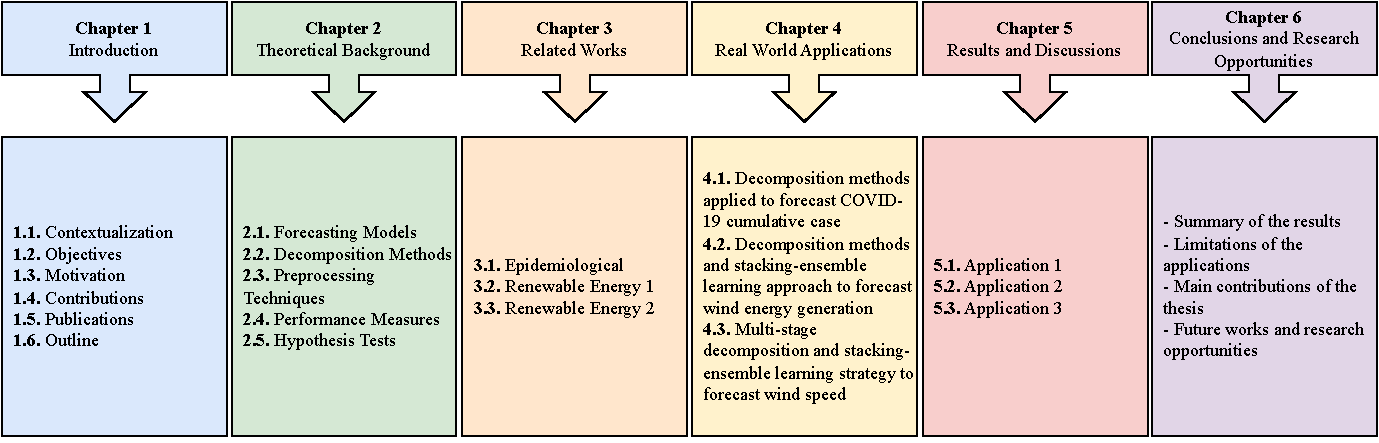
\includegraphics[width=1.5\textwidth]{Media/thesis-outline-transposed.pdf}
    \caption{Thesis structure}
    \label{fig:outline}
    \source{Author (2023)}
\end{figure}
\end{landscape}